% 图 26.2 —— **结构化重画**（2026-09-25，替换掉 `checks/emit_hand.py` 的逐段拟合稿）
%%
% 结构：3 条轴（上、下=x轴、左=y轴）+ 1 条粗竖线 x₀×Y + 5 个矩形 U_i×V_i + 1 条 45° 阴影管带 W×Y + 2 条波浪曲线（开集 N 的边界）+ 2 只小钩 + 1 支弯箭头 + 1 个花括号 + 标签 N W X y
%%
% 旧版是**描摹**：把每一段笔画单独拟合后发出来，连「箭头头」都被当成"一条很粗的短线"描
%   （图 81.5 上一度出现 `\draw[line width=7.0pt] (586,277)--(586,270);` 这种 7px 长的疙瘩），
%   渲染出来是黑疙瘩而不是箭头。本版改成**看懂结构后用 TikZ 画**。
%%
% 做法、约定、已踩过的坑 → `＜工作区＞\checks\redraw\README_重画流程.md`
% 本图圆/椭圆的中心与半径、标签的文字与位置，沿用 probe 的脚手架（那部分它是对的）。
%%
% ⚠ 本图 tikzpicture 是 y=-1pt（**y 翻转**）⇒ `arc` 的角向"递减"才是屏幕逆时针；
%   同一根线上的多段弧必须同向。改完务必拿原书并排、放大核箭头朝向。
%%
\documentclass[12pt]{standalone}
\usepackage{fontspec}
\setsansfont{Arial}
\newfontfamily\mfallback{DejaVu Sans}
\usepackage{tikz}
\usetikzlibrary{arrows.meta}
\begin{document}
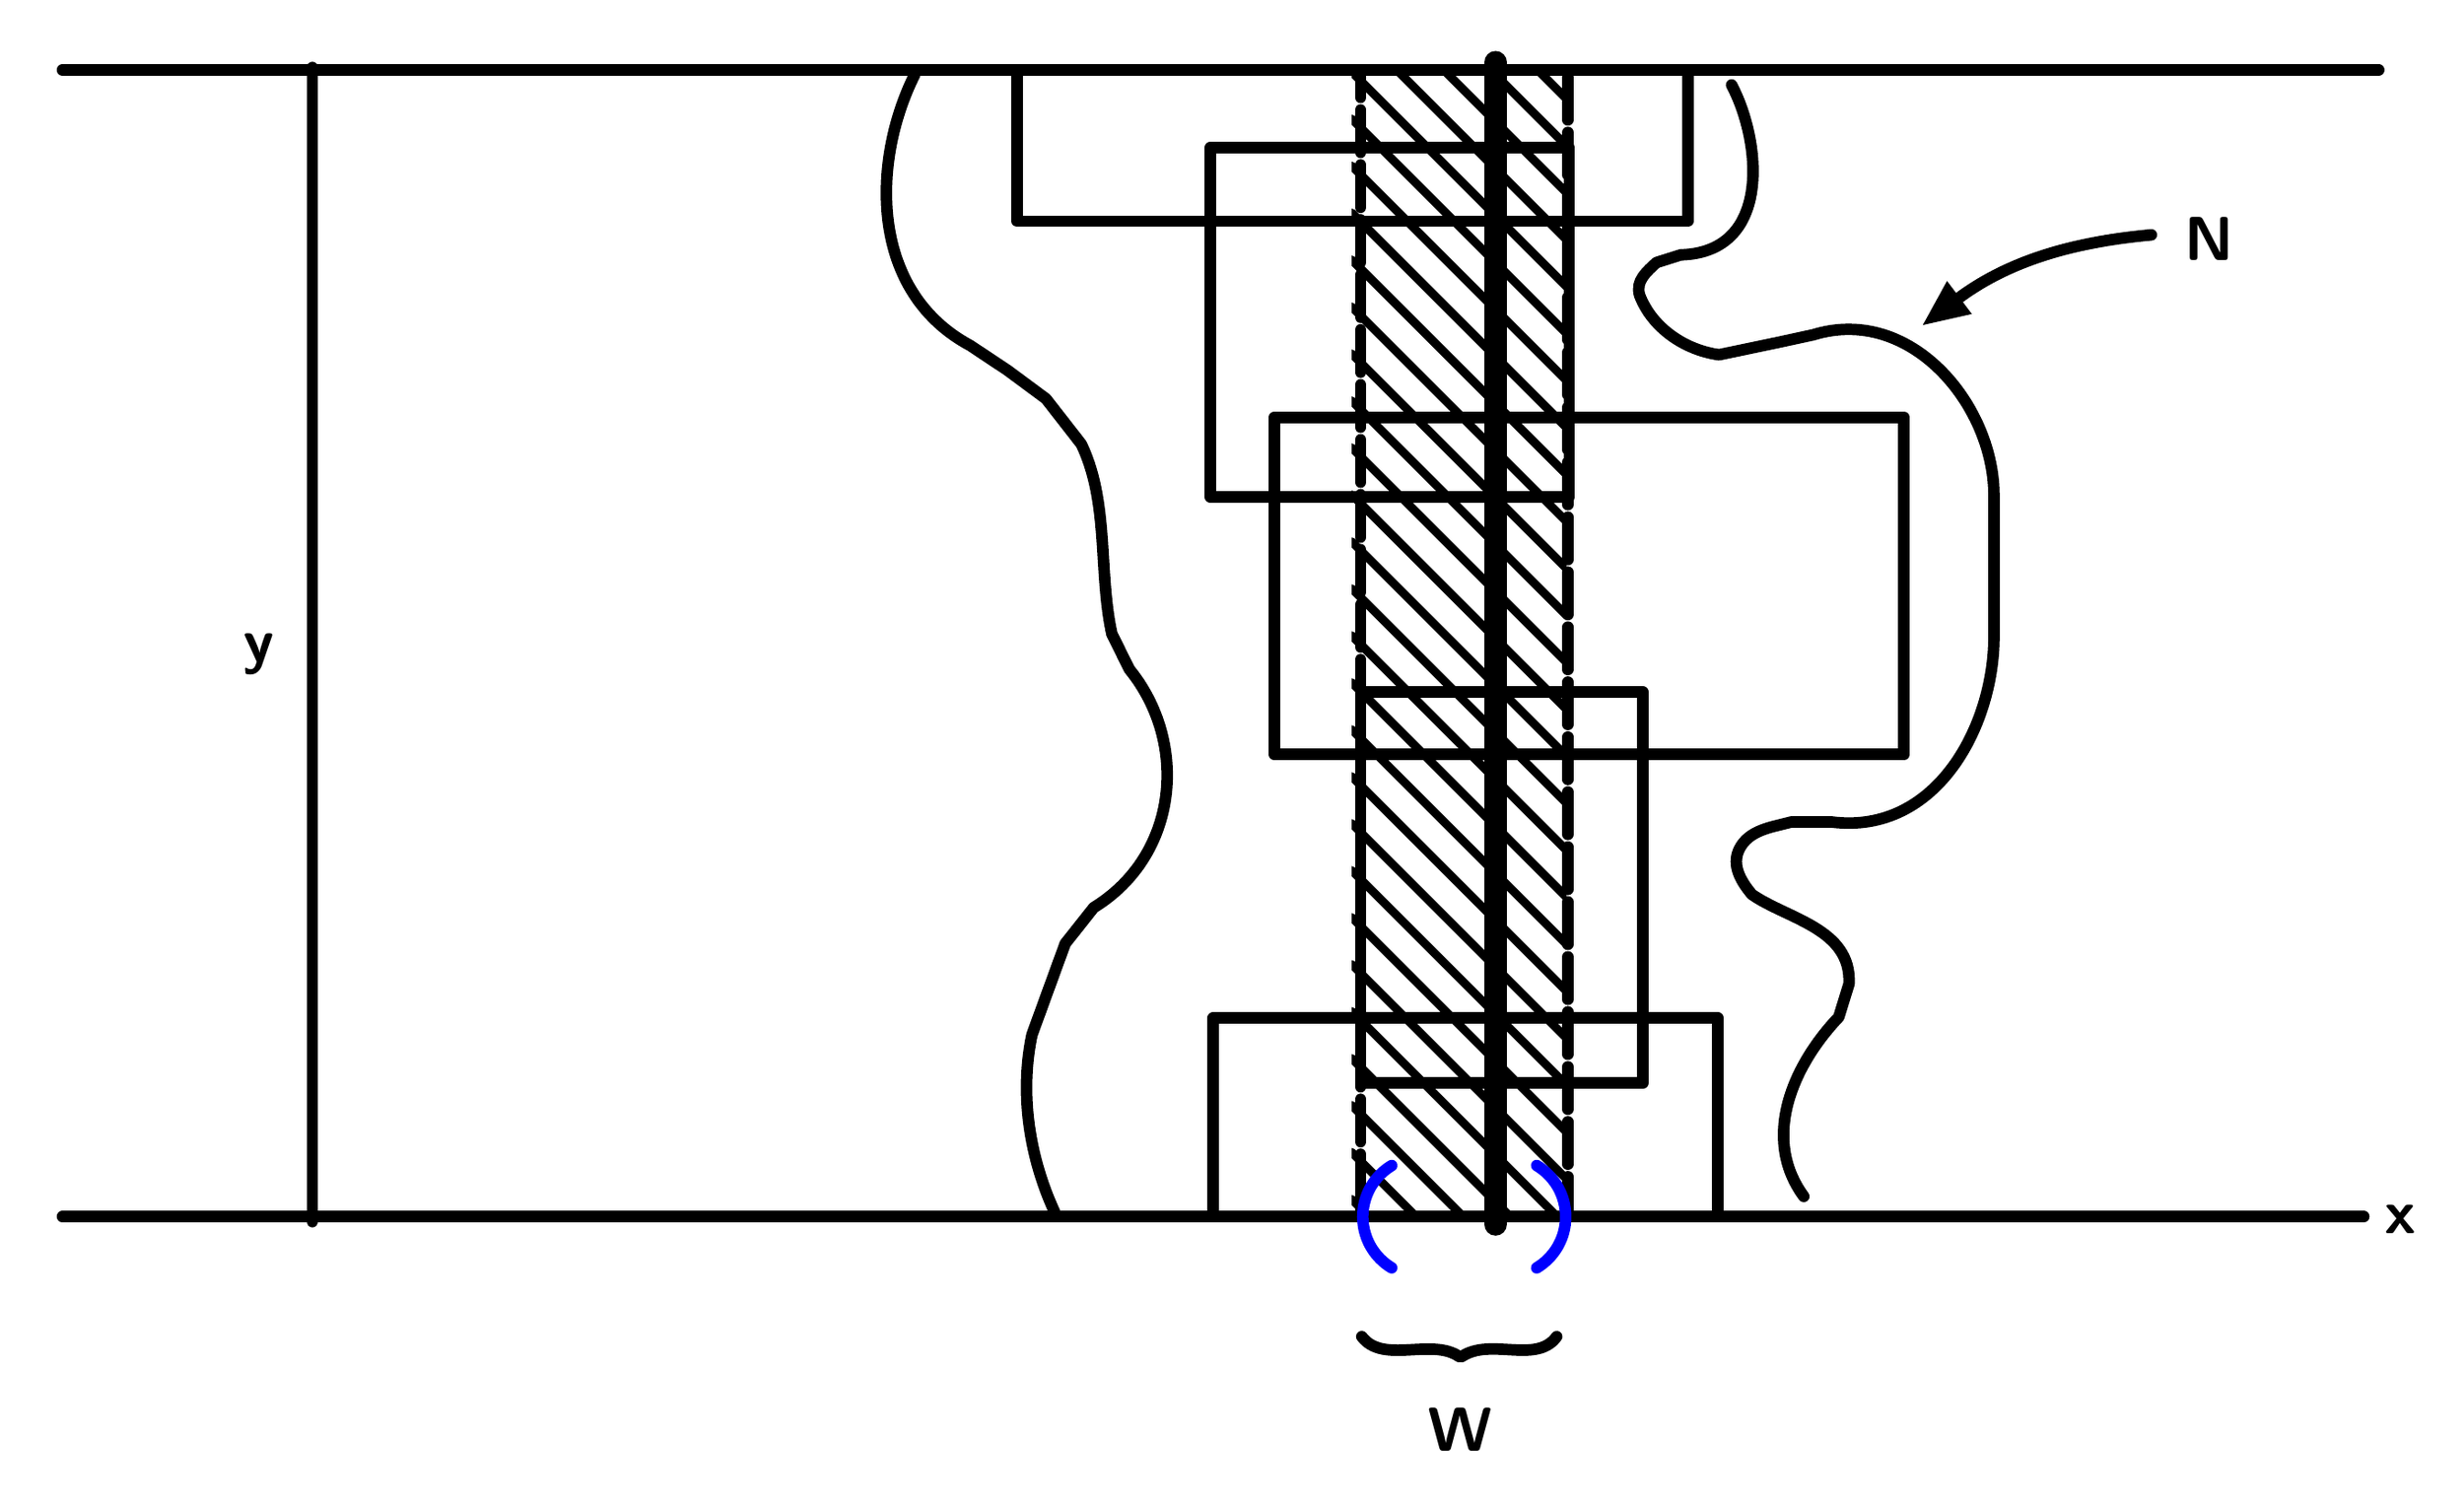
\begin{tikzpicture}[x=1pt, y=-1pt, line width=4.6pt, line cap=round, line join=round]
  % 箭头头规格: 本图用 README §3.5 的垂向剖面法实测 = 峰值宽 15、沿轴长 19
  \def\arr{-{Triangle[width=15pt,length=19pt]}}

  % ════ 边框 / 坐标轴 ════
  \draw (15,18) -- (942,18);            % 上边界
  \draw (15,477) -- (936,477);          % 下边界（x 轴）
  \draw (115,17) -- (115,479);          % 左边界（y 轴）

  % ════ 截面 x0 × Y（粗线）════
  \draw[line width=9.2pt] (588.5,15) -- (588.5,480);

  % ════ 基元素 U_i × V_i（5 个矩形）════
  \draw (397,18)    rectangle (665.5,78.5);
  \draw (474.5,49)  rectangle (618,189);
  \draw (500,157)   rectangle (752,292);
  \draw (534.5,267) rectangle (647.5,423.5);
  \draw (475.5,397.5) rectangle (677.5,477);

  % ════ 管 W × Y：45° 阴影族（等距平行线, 间距 18.8, 相位实测）+ 两侧虚线界 ════
  \begin{scope}
    \clip (531,18) rectangle (617,477);
    \foreach \k in {0,...,31}{%
      \pgfmathsetmacro\cc{4.6+18.8*\k}%
      \draw[line width=3.4pt] (531,{531-\cc}) -- (617,{617-\cc});}
  \end{scope}
  \draw[dash pattern=on 17pt off 5pt, dash phase=6pt]  (534.5,18) -- (534.5,477);
  \draw[dash pattern=on 17pt off 5pt, dash phase=-3pt] (617.5,18) -- (617.5,477);

  % ════ 开集 N 的边界（两条波浪线）════
  \draw (412,475) .. controls (402.2,453.6) and (397.9,428.4) .. (403,404.2)
     -- (416.3,367.7) -- (427.7,353.3)
     .. controls (461.7,332.4) and (465.9,287.3) .. (442,257.9)
     -- (435,243.8)
     .. controls (429.5,218.9) and (434,191) .. (422.7,167.7)
     -- (408.6,149.6) -- (393.2,138.2) -- (378.3,128.3)
     .. controls (338.2,106.8) and (338.5,55.3) .. (356,20);

  \draw (711.9,468.9) .. controls (694.6,445.3) and (707.8,416.1) .. (725.9,397.1)
     -- (730,383.8)
     .. controls (731.1,361.6) and (705.1,357.8) .. (691.1,348)
     .. controls (686.9,342.9) and (682.9,336.6) .. (686,330)
     .. controls (690,321.9) and (699.5,321.1) .. (706.9,319)
     -- (722.9,319)
     .. controls (765.6,324.5) and (788.6,279.3) .. (788,243.3)
     -- (788,187.7)
     .. controls (787.6,151.8) and (754.6,112) .. (715.7,124)
     -- (701.9,127) -- (678,132)
     .. controls (664.6,130.2) and (651.3,121.5) .. (646.2,108.2)
     .. controls (644.4,102.4) and (649.2,98.6) .. (652.9,95.1)
     -- (662.7,92)
     .. controls (699.2,91) and (695,46.7) .. (683,24);

  % ════ 区间 W 的**开区间端帽**（左右各一）════
  %% ！它们**不是自由笔画，各自就是一条圆弧** —— 和 图 3.3 里标开区间端点是同一套记号。
  %% 2026-09-25 第二次重做：上一版我拿三次贝塞尔去拟合一整段约 143° 的弧，最小二乘
  %%   只能凑出「一段直线 + 一个脚」的假形状，于是误判成"手画的犄角"、还去描它的墨迹。
  %%   正确做法是**按圆弧拟合**：逐行提中心线做最小二乘圆，圆度残差 ≤1.2 画布单位。
  %% 实测：圆心 (559.3,477)、半径 23.9 —— **圆心落在 x 轴上**。
  %% ⚠ 对称是**两组**，缺一不可：
  %%   ① 左右：两个端帽关于带中心 x=576 互为镜像（右端帽圆心 592.7）；
  %%   ② **上下**：每个端帽**关于 x 轴**上下对称 —— 它是绕在 x 轴这个"区间杆"的端头上的，
  %%      不能只往上翘一边（我第一版就是这么错的：一弧 115°→200°，下面长上面短）。
  %%      轴线在 477，所以角向取 121°→239°（中值 180°=x 轴方向），上下各扫 59°。
  %% 画法照 图 3.3 的开区间端帽写法：`(圆心) ++(角:半径) arc[start,end,radius]`。
  %% 颜色用**蓝色**：原书是纯灰度（我核过整页彩度=0），蓝色是这里**刻意加**的，
  %%   目的就是把这几个端点画成"W 是开区间"的几何记号，让人一眼认出来。
  \draw[blue, line width=4.6pt] (559.3,477) ++(121:23.9) arc[start angle=121, end angle=239, radius=23.9];
  \draw[blue, line width=4.6pt] (592.7,477) ++(301:23.9) arc[start angle=301, end angle=419, radius=23.9];

  % ════ 由 N 指向边界（N 的标注箭头）════
  \draw[\arr] (851,84) .. controls (823.2,86.6) and (795.7,92.9) .. (759,120.5);

  % ════ W 的花括号 ════
  \draw (574,533) .. controls (562.9,525.3) and (543.5,536.2) .. (535,525);
  \draw (575,533) .. controls (586.5,525.2) and (604.9,536.2) .. (613,525);

  % ════ 标签 ════
  \node[anchor=center,inner sep=0pt,font=\fontsize{29.6}{37.0}\selectfont] at (874.2,85.5) {\textsf{\textbf{\textit{N}}}};
  \node[anchor=center,inner sep=0pt,font=\fontsize{29.8}{37.3}\selectfont] at (93.7,251.7) {\textsf{\textbf{\textit{y}}}};
  \node[anchor=center,inner sep=0pt,font=\fontsize{38.9}{48.7}\selectfont] at (950.8,478.1) {\textsf{\textbf{\textit{x}}}};
  \node[anchor=center,inner sep=0pt,font=\fontsize{28.0}{35.0}\selectfont] at (574.7,562.4) {\textsf{\textbf{\textit{W}}}};

  % 钉死画布：超出画布的图元不允许把页面撑大
  \path[use as bounding box] (0,0) rectangle (966,582);
\end{tikzpicture}
\end{document}
